\section{Grafik Kompleksitas dan Visualisasi}

Memahami kompleksitas algoritma sangat penting untuk memilih algoritma yang tepat untuk masalah tertentu. Grafik kompleksitas membantu visualisasi performa algoritma pada berbagai ukuran input.

\subsection{Grafik Kompleksitas Waktu}

\begin{center}
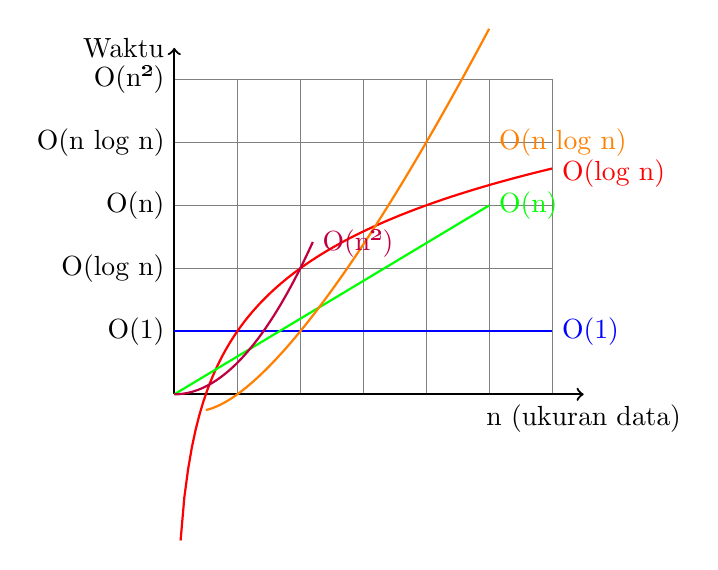
\begin{tikzpicture}[scale=0.8]
  % Grid
  \draw[gray, very thin] (0,0) grid (6,5);
  
  % Axes
  \draw[thick, ->] (0,0) -- (6.5,0) node[anchor=north] {n (ukuran data)};
  \draw[thick, ->] (0,0) -- (0,5.5) node[anchor=east] {Waktu};
  
  % Labels
  \node[anchor=east] at (0,1) {O(1)};
  \node[anchor=east] at (0,2) {O(log n)};
  \node[anchor=east] at (0,3) {O(n)};
  \node[anchor=east] at (0,4) {O(n log n)};
  \node[anchor=east] at (0,5) {O(n²)};
  
  % O(1) - Constant
  \draw[blue, thick] (0,1) -- (6,1);
  \node[blue, anchor=west] at (6,1) {O(1)};
  
  % O(log n) - Logarithmic
  \draw[red, thick, domain=0.1:6, samples=100] plot (\x, {1 + ln(\x)/ln(2)});
  \node[red, anchor=west] at (6,3.5) {O(log n)};
  
  % O(n) - Linear
  \draw[green, thick] (0,0) -- (5,3);
  \node[green, anchor=west] at (5,3) {O(n)};
  
  % O(n log n)
  \draw[orange, thick, domain=0.5:5, samples=100] plot (\x, {0.5*\x*ln(\x)/ln(2)});
  \node[orange, anchor=west] at (5,4) {O(n log n)};
  
  % O(n²) - Quadratic
  \draw[purple, thick, domain=0:2.2, samples=100] plot (\x, {0.5*\x*\x});
  \node[purple, anchor=west] at (2.2,2.4) {O(n²)};
\end{tikzpicture}
\end{center}

\subsection{Tabel Perbandingan Komprehensif}

\begin{table}[h]
\centering
\small
\begin{tabular}{|>{\raggedright\arraybackslash}p{2.5cm}|>{\raggedright\arraybackslash}p{2cm}|>{\raggedright\arraybackslash}p{2cm}|>{\raggedright\arraybackslash}p{2cm}|>{\raggedright\arraybackslash}p{3cm}|}
\hline
\textbf{Algoritma} & \textbf{Waktu} & \textbf{Space} & \textbf{Stabil} & \textbf{Kapan Digunakan} \\
\hline
Bubble Sort & O(n²) & O(1) & Ya & Data kecil, sudah hampir terurut \\
\hline
Selection Sort & O(n²) & O(1) & Tidak & Data kecil, meminimalkan pertukaran \\
\hline
Linear Search & O(n) & O(1) & Ya & Data tidak terurut, pencarian tunggal \\
\hline
Binary Search & O(log n) & O(1) & Ya & Data terurut, pencarian berulang \\
\hline
\end{tabular}
\caption{Perbandingan Lengkap Algoritma Sorting dan Searching}
\end{table}

\subsection{Visualisasi Proses Binary Search}

\textbf{Contoh Pencarian 23 dalam [2, 5, 8, 12, 16, 23, 38, 56, 72, 91]}

\begin{center}
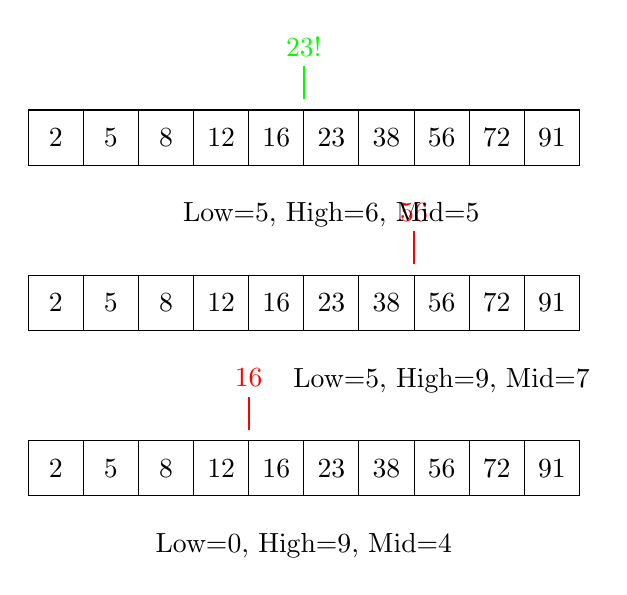
\begin{tikzpicture}[scale=0.7]
  % Initial array
  \foreach \x/\val in {0/2, 1/5, 2/8, 3/12, 4/16, 5/23, 6/38, 7/56, 8/72, 9/91} {
    \draw (\x,0) rectangle (\x+1,1);
    \node at (\x+0.5,0.5) {\val};
  }
  \node[below] at (5,-0.5) {Low=0, High=9, Mid=4};
  \draw[red, thick] (4,1.2) -- (4,1.8);
  \node[red, above] at (4,1.8) {16};
  
  % Step 2
  \foreach \x/\val in {0/2, 1/5, 2/8, 3/12, 4/16, 5/23, 6/38, 7/56, 8/72, 9/91} {
    \draw (\x,3) rectangle (\x+1,4);
    \node at (\x+0.5,3.5) {\val};
  }
  \node[below] at (7.5,2.5) {Low=5, High=9, Mid=7};
  \draw[red, thick] (7,4.2) -- (7,4.8);
  \node[red, above] at (7,4.8) {56};
  
  % Step 3
  \foreach \x/\val in {0/2, 1/5, 2/8, 3/12, 4/16, 5/23, 6/38, 7/56, 8/72, 9/91} {
    \draw (\x,6) rectangle (\x+1,7);
    \node at (\x+0.5,6.5) {\val};
  }
  \node[below] at (5.5,5.5) {Low=5, High=6, Mid=5};
  \draw[green, thick] (5,7.2) -- (5,7.8);
  \node[green, above] at (5,7.8) {23!};
\end{tikzpicture}
\end{center}

\subsection{Animasi Bubble Sort}

\textbf{Proses Bubble Sort pada [64, 34, 25, 12, 22]:}

\begin{center}
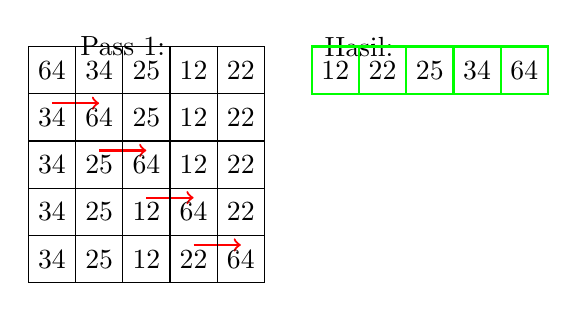
\begin{tikzpicture}[scale=0.6]
  % Pass 1
  \node at (2,8) {Pass 1:};
  \foreach \x/\val in {0/64, 1/34, 2/25, 3/12, 4/22} {
    \draw (\x,7) rectangle (\x+1,8);
    \node at (\x+0.5,7.5) {\val};
  }
  \draw[red, thick, ->] (0.5,6.8) -- (1.5,6.8);
  
  % After swap 1
  \foreach \x/\val in {0/34, 1/64, 2/25, 3/12, 4/22} {
    \draw (\x,6) rectangle (\x+1,7);
    \node at (\x+0.5,6.5) {\val};
  }
  \draw[red, thick, ->] (1.5,5.8) -- (2.5,5.8);
  
  % After swap 2
  \foreach \x/\val in {0/34, 1/25, 2/64, 3/12, 4/22} {
    \draw (\x,5) rectangle (\x+1,6);
    \node at (\x+0.5,5.5) {\val};
  }
  \draw[red, thick, ->] (2.5,4.8) -- (3.5,4.8);
  
  % After swap 3
  \foreach \x/\val in {0/34, 1/25, 2/12, 3/64, 4/22} {
    \draw (\x,4) rectangle (\x+1,5);
    \node at (\x+0.5,4.5) {\val};
  }
  \draw[red, thick, ->] (3.5,3.8) -- (4.5,3.8);
  
  % End of pass 1
  \foreach \x/\val in {0/34, 1/25, 2/12, 3/22, 4/64} {
    \draw (\x,3) rectangle (\x+1,4);
    \node at (\x+0.5,3.5) {\val};
  }
  
  % Final result
  \node at (7,8) {Hasil:};
  \foreach \x/\val in {0/12, 1/22, 2/25, 3/34, 4/64} {
    \draw[green, thick] (\x+6,7) rectangle (\x+7,8);
    \node at (\x+6.5,7.5) {\val};
  }
\end{tikzpicture}
\end{center}

\subsection{Analisis Performa Real-world}

\begin{table}[h]
\centering
\small
\begin{tabular}{|>{\raggedright\arraybackslash}p{2.5cm}|>{\raggedright\arraybackslash}p{2cm}|>{\raggedright\arraybackslash}p{2cm}|>{\raggedright\arraybackslash}p{2cm}|}
\hline
\textbf{Ukuran Data} & \textbf{Bubble Sort} & \textbf{Selection Sort} & \textbf{Binary Search} \\
\hline
10 elemen & 0.001 ms & 0.001 ms & 0.0001 ms \\
\hline
100 elemen & 0.1 ms & 0.1 ms & 0.0002 ms \\
\hline
1,000 elemen & 10 ms & 10 ms & 0.0003 ms \\
\hline
10,000 elemen & 1000 ms & 1000 ms & 0.0004 ms \\
\hline
100,000 elemen & 100,000 ms & 100,000 ms & 0.0005 ms \\
\hline
\end{tabular}
\caption{Estimasi Waktu Eksekusi (asumsi 1 operasi = 1\,\textmu s)}
\end{table}

Visualisasi ini membantu mahasiswa memahami mengapa pemilihan algoritma sangat penting dalam pengembangan perangkat lunak yang efisien.
